\documentclass[border=15pt,tikz]{standalone}
\usepackage{amsmath}
\usetikzlibrary{arrows.meta, fit, positioning, backgrounds}
\usepackage[outline]{contour}
\contourlength{1.4pt}

\usepackage{helvet}
\renewcommand{\familydefault}{\sfdefault}

% --- COLOR DEFINITIONS ---
\usepackage{xcolor}
\colorlet{myred}{red!80!black}
\colorlet{myblue}{blue!80!black}
\colorlet{mygreen}{green!60!black}
\colorlet{myorange}{orange!70!red!60!black}
\colorlet{mydarkred}{red!30!black}
\colorlet{mydarkblue}{blue!40!black}
\colorlet{mydarkgreen}{green!30!black}

% --- STYLES ---
\tikzset{
  >=latex,
  base node/.style={thick, circle, minimum size=28pt, inner sep=1pt, align=center, font=\footnotesize},
  node graph/.style={base node, draw=mygreen!40!black, fill=mygreen!15},
  node gcn/.style={base node, draw=myblue!40!black, fill=myblue!15},
  node mlp/.style={base node, draw=myorange!40!black, fill=myorange!15},
  node out/.style={base node, draw=myred!40!black, fill=myred!15},
  dipole edge/.style={->, thick, mydarkgreen, shorten >=2pt, shorten <=2pt},
  msg edge/.style={->, thick, mydarkblue, shorten >=2pt, shorten <=2pt},
  dense edge/.style={thick, mydarkblue, opacity=0.3},
  flow arrow/.style={->, thick, line width=1.5pt, draw=black!60},
  label/.style={font=\small\bfseries, align=center},
  desc/.style={font=\scriptsize, align=center, text=black!80},
  box/.style={draw, thick, rounded corners=6pt, inner sep=14pt, fill opacity=0.05}
}

\begin{document}

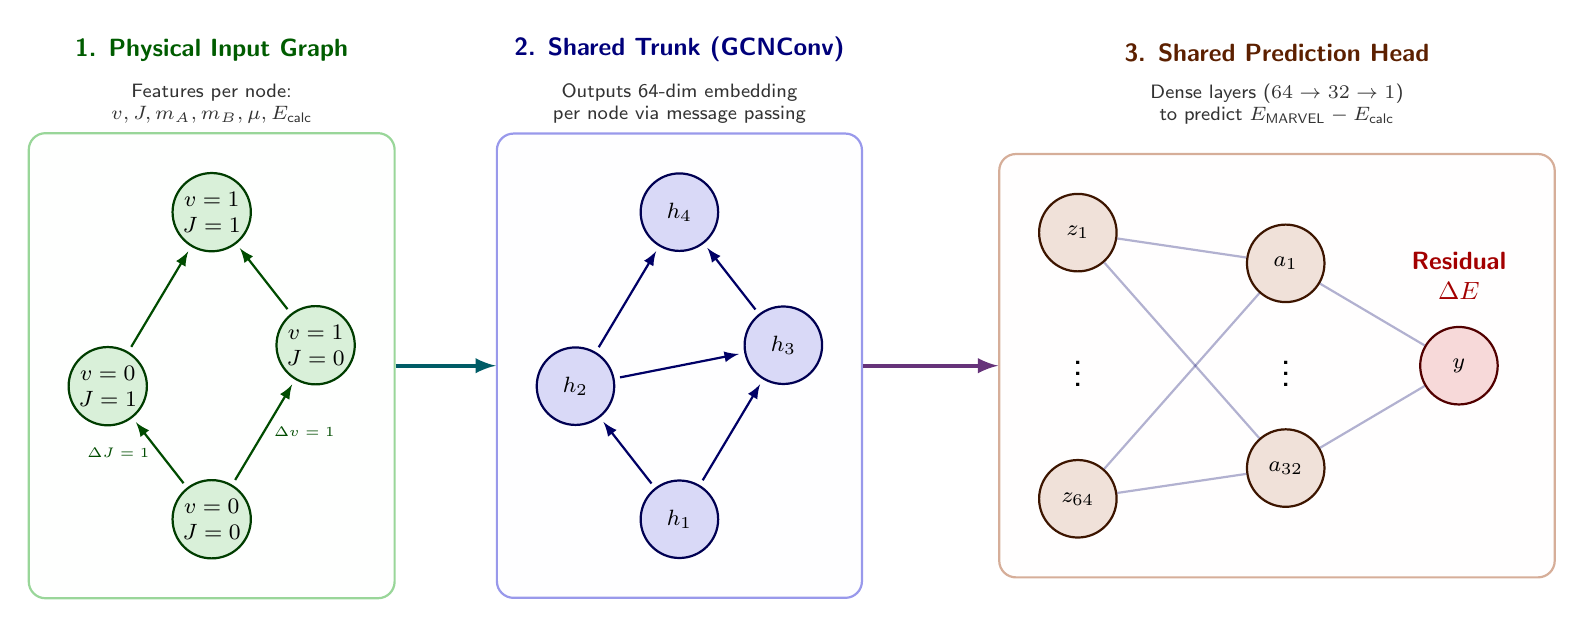
\begin{tikzpicture}[x=2.2cm, y=1.3cm, font=\sffamily]

  % =================================================================================
  % SECTION 1: PHYSICAL INPUT GRAPH
  % =================================================================================
  
  % Hierarchical arrangement by energy/states (lowest at bottom, highest at top)
  \node[node graph] (G1) at (0.8, 1.0) {$v=0$\\$J=0$};
  \node[node graph] (G2) at (0.2, 2.3) {$v=0$\\$J=1$};
  \node[node graph] (G3) at (1.4, 2.7) {$v=1$\\$J=0$};
  \node[node graph] (G4) at (0.8, 4.0) {$v=1$\\$J=1$};
  
  % Physical transition edges
  \draw[dipole edge] (G1) -- (G2) node[midway, left, font=\tiny] {$\Delta J=1$};
  \draw[dipole edge] (G1) -- (G3) node[midway, right, font=\tiny] {$\Delta v=1$};
  \draw[dipole edge] (G2) -- (G4);
  \draw[dipole edge] (G3) -- (G4);

  % Bounding Box around the Graph
  \begin{pgfonlayer}{background}
    \node[box, fit=(G1) (G2) (G3) (G4), fill=mygreen!5, draw=mygreen!40] (box-input) {};
  \end{pgfonlayer}
  
  % Integrated Title and Subtitle positioned cleanly above the box
  \node[label, mygreen!60!black, above=22pt of box-input.north] (Title1) {1. Physical Input Graph};
  \node[desc, below=1pt of Title1] {Features per node:\\$v, J, m_A, m_B, \mu, E_{\text{calc}}$};


  % =================================================================================
  % SECTION 2: SHARED TRUNK (GCNConv)
  % =================================================================================
  
  % Mirrored geometric layout, labeled strictly ascending by height
  \node[node gcn] (H1) at (3.5, 1.0) {$h_1$};
  \node[node gcn] (H2) at (2.9, 2.3) {$h_2$};
  \node[node gcn] (H3) at (4.1, 2.7) {$h_3$};
  \node[node gcn] (H4) at (3.5, 4.0) {$h_4$};

  % Message passing links sharing physics along the graph topology
  \draw[msg edge] (H1) -- (H2);
  \draw[msg edge] (H1) -- (H3);
  \draw[msg edge] (H2) -- (H4);
  \draw[msg edge] (H3) -- (H4);
  \draw[msg edge] (H2) -- (H3);

  % Bounding Box around the Trunk
  \begin{pgfonlayer}{background}
    \node[box, fit=(H1) (H2) (H3) (H4), fill=myblue!5, draw=myblue!40] (box-trunk) {};
  \end{pgfonlayer}
  
  % Integrated Title and Subtitle positioned cleanly above the box
  \node[label, myblue!60!black, above=22pt of box-trunk.north] (Title2) {2. Shared Trunk (GCNConv)};
  \node[desc, below=1pt of Title2] {Outputs 64-dim embedding\\per node via message passing};


  % =================================================================================
  % SECTION 3: SHARED PREDICTION HEAD (Explicit DNN Topology)
  % =================================================================================
  
  % --- Layer 1: GCN Output / MLP Input (64 nodes) ---
  \node[node mlp] (MLP_In1) at (5.8, 3.8) {$z_1$};
  \node[node mlp] (MLP_In2) at (5.8, 1.2) {$z_{64}$};
  \path (MLP_In1) -- (MLP_In2) node[midway, font=\Large] {$\vdots$};
  
  % --- Layer 2: Hidden Dense Layer (32 nodes) ---
  \node[node mlp] (MLP_H1) at (7.0, 3.5) {$a_1$};
  \node[node mlp] (MLP_H2) at (7.0, 1.5) {$a_{32}$};
  \path (MLP_H1) -- (MLP_H2) node[midway, font=\Large] {$\vdots$};
  
  % --- Layer 3: Single Scalar Output Node ---
  \node[node out] (MLP_Out) at (8.0, 2.5) {$y$};
  
  % Fully Connected Dense Edges (Layer 1 -> Layer 2)
  \draw[dense edge] (MLP_In1) -- (MLP_H1);
  \draw[dense edge] (MLP_In1) -- (MLP_H2);
  \draw[dense edge] (MLP_In2) -- (MLP_H1);
  \draw[dense edge] (MLP_In2) -- (MLP_H2);
  
  % Fully Connected Dense Edges (Layer 2 -> Output)
  \draw[dense edge] (MLP_H1) -- (MLP_Out);
  \draw[dense edge] (MLP_H2) -- (MLP_Out);
  
  % Final targeted residual output tag
  \node[label, above=6pt of MLP_Out, font=\small\bfseries, text=myred!80!black] (Target) {Residual\\$\Delta E$};

  % Bounding Box around the explicit DNN Head nodes
  \begin{pgfonlayer}{background}
    \node[box, fit=(MLP_In1) (MLP_In2) (MLP_Out) (Target), fill=myorange!5, draw=myorange!40] (box-head) {};
  \end{pgfonlayer}

  % Title positioned above the box
  \node[label, myorange!60!black, at={(box-head.north |- Title2.south)}, anchor=south] (Title3) {3. Shared Prediction Head};
  \node[desc, below=1pt of Title3] {Dense layers ($64 \to 32 \to 1$)\\to predict $E_{\text{MARVEL}} - E_{\text{calc}}$};


  % =================================================================================
  % MACRO FLOW CONNECTIONS (Solid Box-to-Box Arrows)
  % =================================================================================
  
  \draw[flow arrow, draw=mygreen!60!blue]  (box-input.east) -- (box-trunk.west);
  \draw[flow arrow, draw=myblue!60!orange] (box-trunk.east) -- (box-head.west);

\end{tikzpicture}

\end{document}